% Preamble
% Compile with XeLaTeX

\documentclass[11pt,oneside,a4paper]{article} % no titlepage
\usepackage{preamble}
\usepackage{enumitem}
\graphicspath{{PIC/}}
%%%%%%%%%%%%%%%%%%%%%%%%%%%%%%%%%%%%%%%%%%%%%%%%%%%%%%%%%%%%%%%%%%%%%%%%%%%%%%%%%%%%%%
\begin{document}

\sidebar{sideBarColor!25}
\simpleheader{titleBackColor}{Grover}{Aruquipa}{PhD Candidate \textbar\ Parallel Robotics}{white}

% Start Minipages
\vspace*{3.49cm}
\adjustbox{valign=t}{\begin{minipage}{7.3cm}
\vspace*{1.2cm}

% Picture
\begin{center}
\begin{tikzpicture}
\node[
circle,
minimum size=\cvPictureWidth,
path picture={
\node at (path picture bounding box.center){
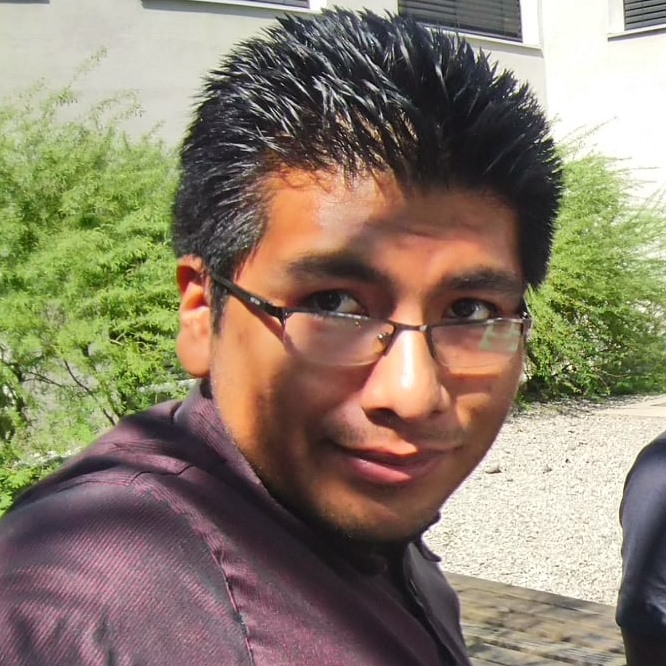
\includegraphics[width=\cvPictureWidth]{Picture.jpg}
};
}]
{};
\end{tikzpicture}
\end{center}

%%%%%%%%%%%%%%%%%%%%%%%%%%%%%%%%%%%%%%%%%%%%%%%%%%%%
% Profile section
\ruleline{\textbf{About me}}
I am a mechatronics engineer and PhD candidate in Mechanical Engineering at Universit\'e Laval (Qu\'ebec, Canada).
My research focuses on advanced parallel robots with kinematic redundancy, \textbf{unlimited rotations}, and \textbf{integrated grasping capabilities}, with an emphasis on kinematic modeling, workspace/singularity analysis, and collision-free design for high-precision manipulation.

%%%%%%%%%%%%%%%%%%%%%%%%%%%%%%%%%%%%%%%%%%%%%%%%%%%%
% Contact Section
\ruleline{\textbf{Contact}}
\begin{tikzpicture}[every node/.style={inner sep=0pt, outer sep=0pt}]
\matrix[
column 1/.style={anchor=center,contactIcon},
column 2/.style={anchor=west,align=left,contactIcon},
column sep=5pt,
row sep=5pt] (contact) {
\node{\faMale}; & \node{Date of birth: 09/09/1995};\\
\node{\faEnvelope}; & \node{\href{mailto:grover.aruquipa-aruquipa.1@ulaval.ca}{grover.aruquipa-aruquipa.1@ulaval.ca}};\\
\node{\faEnvelopeO}; & \node{\href{mailto:grover.aruquipa.9@gmail.com}{grover.aruquipa.9@gmail.com}};\\
\node{\faPhone}; & \node{+33 6 29 77 92 25};\\
\node{\faMapMarker}; & \node{Qu\'ebec, QC, Canada};\\
\node{\faLinkedinSquare}; & \node{\href{https://www.linkedin.com/in/grover-aruquipa-996917126}{linkedin.com/in/grover-aruquipa-996917126}};\\
\node{\aiResearchGateSquare}; & \node{\href{https://www.researchgate.net/profile/Grover-Aruquipa}{ResearchGate: Grover Aruquipa}};\\
\node{\aiOrcid}; & \node{\href{https://orcid.org/0000-0003-0243-3187}{ORCID: 0000-0003-0243-3187}};\\
\node{\faGithub}; & \node{\href{https://groveraruquipa.github.io/}{groveraruquipa.github.io}};\\
\node{\faGear}; & \node{\href{https://grabcad.com/grover.aruquipa.aruquipa-1/models}{GrabCAD: Grover Aruquipa}};\\
};
\end{tikzpicture}

%%%%%%%%%%%%%%%%%%%%%%%%%%%%%%%%%%%%%%%%%%%%%%%%%%%%
% Languages
\ruleline{\textbf{Languages}}
\begin{tikzpicture}[every node/.style={inner sep=0pt, outer sep=0pt}]
\matrix[
column 1/.style={anchor=center,contactIcon},
column 2/.style={anchor=west,align=left,contactIcon},
column sep=5pt,
row sep=5pt] (langs) {
\node{\flag{England.png}}; & \node{English --- Full Professional Proficiency};\\
\node{\flag{Spain.png}}; & \node{Spanish --- Native};\\
\node{\flag{France.png}}; & \node{French --- Professional Working Proficiency};\\
};
\end{tikzpicture}

%%%%%%%%%%%%%%%%%%%%%%%%%%%%%%%%%%%%%%%%%%%%%%%%%%%%
% QR Code
\begin{center}

\includegraphics[width=3.5cm]{PIC/qrdelete1.png}
\end{center}

\end{minipage}}%
\hfill
%%%%%%%%%%%%%%%%%%%%%%%%%%%%%%%%%%%%%%%%%%%%%%%%%%%%%%%%%
%%%%% MAIN SECTION (PAGE 1) %%%%%%%%%%%%%%%%%%%%
\adjustbox{valign=t}{\begin{minipage}{11.3cm}
\vspace*{1cm}

% ==========================================================
% 1) EDUCATION
% ==========================================================
\section*{{\faGraduationCap} EDUCATION}

\MySection{2023--2026}{Books.png}{PhD Degree}{PhD in Mechanical Engineering \textit{Universit\'e Laval}}{Qu\'ebec, Canada}
{Dissertation: Kinematically redundant parallel robots with \textbf{unlimited rotations} and \textbf{grasping capabilities}.}
{Supervisor: Prof.\ Cl\'ement Gosselin.}

\vspace*{0.22cm}

\MySection{2021--2023}{Books.png}{Master's Degree}{Universit\'e Bourgogne--Franche-Comt\'e (UBFC)}{Besan\c{c}on, France}
{MSc in Electrical Engineering: Smart Integrated Systems.}
{Specialization: Robotics and Micro-Robotics.}

\vspace*{0.22cm}

\MySection{2022}{Books.png}{Postgraduate Specialization}{Bolivian Catholic University}{La Paz, Bolivia}
{Postgraduate program: Robotics and Automation.}
{Diplomas: Industrial Automation, Internet of Things, Robotics, and Machine Learning. Final project grade: 82/100.}

\vspace*{0.22cm}

\MySection{2014--2019}{Books.png}{Bachelor's Degree}{Bolivian Catholic University}{La Paz, Bolivia}
{BEng in Mechatronics Engineering.}
{Engineering thesis.}

% ==========================================================
% 2) WORK EXPERIENCE
% ==========================================================
\section*{{\faSuitcase} WORK EXPERIENCE}

\MySectionNoPic{2022--2023}{FEMTO-ST (CNRS UMR 6174)}{Besan\c{c}on, France}
{Research Intern (mandatory internship)}
{Research on parallel robots for micro-manipulation applications.}

\vspace*{0.22cm}

\MySectionNoPic{2021}{Sencon Srl}{Remote}
{Computer Vision Engineer}
{Developed computer vision solutions for anomaly detection.}

\vspace*{0.22cm}

\MySectionNoPic{2021}{KTH Royal Institute of Technology}{Sweden}
{Data Scientist}
{Data analysis for environmental impact assessment.}

\vspace*{0.22cm}

\MySectionNoPic{2020}{Hitachi ABB Power Grids (R\&D)}{Zurich, Switzerland}
{Graduate Research Intern}
{Analysis of complex datasets for high-voltage circuit breakers.}

% ==========================================================
% 3) SCHOLARSHIPS & AWARDS
% ==========================================================
\section*{{\faTrophy}\;SCHOLARSHIPS \& AWARDS}
\begin{itemize}[leftmargin=*, itemsep=0.2ex, topsep=0.4ex]
\footnotesize
\item \textbf{ASME SMRDC Design Competition --- 1st Place (Graduate Division), 2025} · ASME IDETC/MR
\item \textbf{Mitacs Globalink Research Award (GRA), 2026} · Mitacs, Canada
\item \textbf{Citoyens du Monde Mobility Grant}, 2023 · Gouvernement du Qu\'ebec
\item \textbf{Delft Summer School --- Screw Theory (2023)} · TU Delft, Netherlands
\item \textbf{UBFC Master Scholarship} · Universit\'e Bourgogne--Franche-Comt\'e (France)
\item \textbf{PhD Scholarship} · Universit\'e Laval (Canada)
\end{itemize}

% ==========================================================
% 4) CERTIFICATIONS (moved BEFORE publications)
% ==========================================================
\section*{{\faCertificate} SELECTED CERTIFICATIONS}
\begin{itemize}[leftmargin=*, itemsep=0.2ex]
\footnotesize
\item IBM AI Engineering --- \textit{Coursera} (2022)
\item Deep Learning Specialization --- \textit{DeepLearning.AI / Coursera} (2020)
\item Reinforcement Learning Specialization --- \textit{University of Alberta} (2020)
\item A Hands-on Introduction to Engineering Simulations --- \textit{Cornell University} (2020)
\end{itemize}

\end{minipage}}%

%%%%%%%%%%%%%%%%%%%%%%%%%%%%%%%%%%%%%%%%%%%%%%%%%%%%%%%%%%%%
% PAGE 2 (Publications + everything else)
\newpage

\sidebar{sideBarColor!25}
\newpageheader{titleBackColor}{Grover}{Aruquipa}{PhD Candidate \faLightbulbO \hspace{1mm} Parallel Robotics}{white}

% %%%%%%%%%%%%%%%%%%%%%%%%%%%%%%%%%% SIDEBAR (PAGE 2) %%%%%%%%%%%%%%%%%%%
\adjustbox{valign=t}{%
\begin{minipage}{7.3cm}
\vspace*{0.4cm}

\ruleline{\textbf{Principal Soft Skills and Strengths}}
\vspace*{-0.5cm}
\begin{center}
\cvtag{Curiosity}\cvtag{Adaptability}\cvtag{Planning \& Organization}\cvtag{Autonomy}\cvtag{Attention to Detail}\cvtag{Problem Solving}\cvtag{Teamwork}
\end{center}

\ruleline{\textbf{Professional Skills}}
\begin{center}
\cvtag{Parallel Robots}\cvtag{Kinematic Modeling}\cvtag{Screw Theory}\cvtag{Control Systems}\cvtag{Robot Design}
\end{center}

\ruleline{\textbf{Other Interests}}
\small
\begin{multicols}{2}
\begin{itemize}
\item Research \flag{Books.png}
\item Programming \flag{Programming.png}
\item Volunteering \flag{volunteer.png}
\item Gym \flag{Gym.png}
\item 3D Printing \flag{3dprint.png}
\item Trading \flag{trading.png}
\item Salsa \flag{Salsa.png}
\end{itemize}
\end{multicols}

\ruleline{\textbf{Download My CV}}
\scriptsize
\centering
Download my full CV via the QR below \aiOverleaf.
\begin{center}
\qrcode[height=2cm]{https://drive.google.com/drive/folders/1BO9pJQW5mQHfAzN5EPvrLMGua0SwvLSq?usp=share_link}
\vspace*{0.4cm}
\end{center}

\end{minipage}
}%
\hfill
%%%%%%%%%%%%%%%%%%%%%%%%%%%%%%%%%%% MAIN (PAGE 2) %%%%%%%%%%%%%%%%%%%%%%%%%
\adjustbox{valign=t}{%
\begin{minipage}{11.3cm}
\vspace*{0.4cm}

% ==========================================================
% PUBLICATIONS (moved to PAGE 2)
% ==========================================================
\section*{{\aiOBP}\;PUBLICATIONS (Selected)}

\publication{Journal (Q1, under review)}{}{
Analysis and Design of a Novel (6+1)-DoF Parallel Robot with Unlimited Rotation and Grasping Capabilities}
{G.~Aruquipa, P.~Lambert, C.~Gosselin}
{Mechanism and Machine Theory (Elsevier)}
{Under review}

\vspace*{0.10cm}

\publication{Journal (Q1, under review)}{}{
Analysis and Design of a Compact Four-DoF Parallel Robot with Unlimited Rotation}
{G.~Aruquipa, V.~Muralidharan, P.~Lambert, R.~Dahmouche, C.~Gosselin}
{Journal of Mechanisms and Robotics (ASME)}
{Under review}

\vspace*{0.10cm}

\publication{Journal Review (submitted)}{}{
Parallel Robots for Grasping Tasks: A Review}
{G.~Aruquipa, P.~Lambert, C.~Gosselin}
{High-impact robotics journal}
{Submitted}

\vspace*{0.12cm}

\publication{Journal (in preparation)}{}{
Geometric Conditions for Collision-Free Unlimited Rotation in Parallel Mechanisms}
{G.~Aruquipa, P.~Lambert, C.~Gosselin}
{Q1 journal target}
{In preparation}

\vspace*{0.10cm}

\publication{Journal (in preparation)}{}{
A 6+2 Kinematically Redundant Parallel Robot with Unlimited Rotations and Integrated Grasping}
{G.~Aruquipa, P.~Lambert, C.~Gosselin}
{Q1 journal target}
{In preparation}

\vspace*{0.12cm}

\publication{Conference (in preparation)}{}{
Kinematic Analysis and Design of a (6+1)-DoF Concentric Parallel Robot with Unlimited Rotation}
{G.~Aruquipa, P.~Lambert, C.~Gosselin}
{IEEE/RSJ IROS 2026}
{In preparation}

\vspace*{0.12cm}

\publication{Conference}{2025}{
Kinematic Analysis and Design of a 9-DoF Parallel Robot with Grasping Capabilities}
{G.~Aruquipa, P.~Lambert, C.~Gosselin}
{CCToMM M3 Symposium}
{DOI: 10.1007/978-3-031-95489-4\_10}

\vspace*{0.10cm}

\publication{Conference}{2022}{
IoT Architecture for Anomaly Detection in Bio-Inspired Manufacturing Systems}
{G.~Aruquipa, F.~Diaz}
{Procedia Computer Science}
{DOI: 10.1016/j.procs.2022.01.242}
% ==========================================================
% REST (PAGE 2)
% ==========================================================
\section*{{\faBook} ACADEMIC SERVICE}
\footnotesize
\begin{itemize}[leftmargin=*, itemsep=0.2ex]
\item Reviewer: \textbf{SETRE} (Sep.\ 2021)
\item Reviewer: \textbf{ISM 2021} --- International Conference on Industry 4.0 and Smart Manufacturing (Nov.\ 2021)
\end{itemize}
\normalsize

\section*{{\faDesktop} TECHNICAL AND COMPUTATIONAL SKILLS}

\ITCcompetence{Computation \& Data}{
\textbf{MATLAB}, \textbf{RStudio}; \textbf{Wolfram Alpha} (intermediate)
}

\vspace*{0.12cm}

\ITCcompetence{Modeling \& CAD}{
\textbf{Simulink}, \textbf{SolidWorks}, \textbf{LabVIEW}; \textbf{PTC Creo}, \textbf{ANSYS}, \textbf{Altium/Proteus} (intermediate)
}

\vspace*{0.12cm}

\ITCcompetence{Robotics \& AI}{
\textbf{ROS/ROS 2}, \textbf{OpenCV}, \textbf{TensorFlow/PyTorch}; \textbf{Dash/Flask/Django}
}

\vspace*{0.12cm}

\ITCcompetence{Writing}{
\textbf{\LaTeX}, \textbf{MS Office} (Excel/Word/PowerPoint)
}

\section*{{\aiImpactstory} VOLUNTEER ACTIVITIES}
\begin{itemize}[leftmargin=*, itemsep=0.2ex]
\footnotesize
\item \textbf{HOPE Worldwide} (2016--2025): Volunteering to support families in need.
\end{itemize}

\end{minipage}}
\end{document}
